\section{}

Briefly describe under what conditions the following are conserved. Give 1 example for each to support your writing. You do not need to write long calculations or more than a couple of sentences in order to achieve full marks for this question.

a) Momentum

b) Energy




\section{}

Consider the system of 2 particles below. At a given instant, one particle is positioned on the z-axis at a distance of $1.5d$ from the origin and has a mass of $4m$, travelling in the x direction at a constant velocity of $v$. The other particle is positioned on the x-axis at distance $d$ from the origin and has a mass of $m$, travelling in the $y$ direction with a velocity of $2v$ while experiencing a force $F$ in the z-direction.

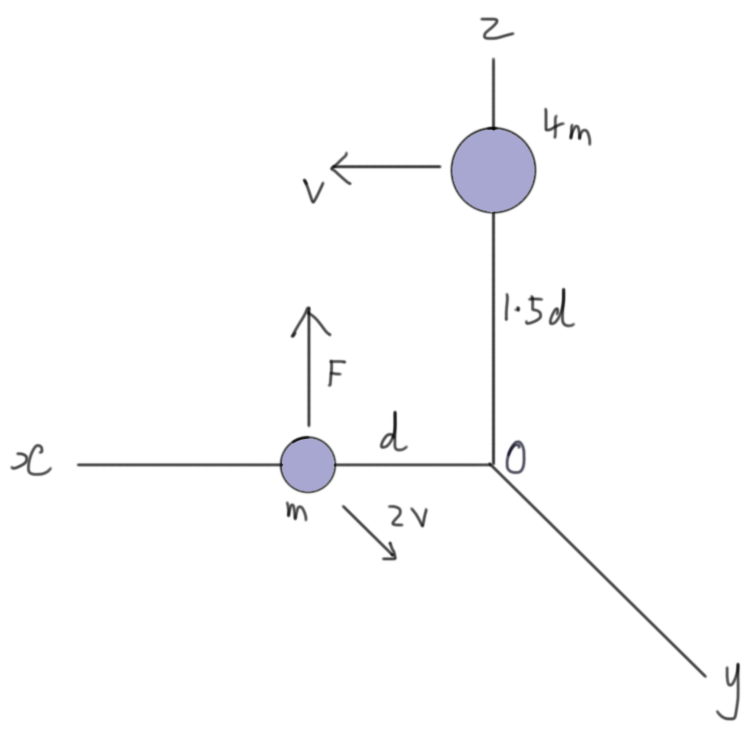
\includegraphics[height=7cm]{particles.png}

a) Determine the centre-of-mass position, velocity and acceleration.

b) Determine the angular momentum and torque about the origin ``O''.

c) Determine the angular momentum about the centre-of-mass of the system.




\section{}
An experimental hovercraft hovers just above the ground by pumping air at atmospheric pressure through the circular induct at $B$ with radius $r_B$ and discharging it horizontally under the skirt $C$ with radius $r_C$. Write an expression for the average air-pressure $P$ under the hovercraft, considering the balance of forces involved. You may consider the specific weight of air to be $\rho$ \si{\kg\per\cubic\meter} and the velocity of air entering the induct $B$ to be $v$ \si{\meter\per\second}.

\emph{Image taken from question 4/50 in book. Not included here for copyright reasons.}




\section{}
Consider a jet aircraft climbing at a constant velocity $v$ at an angle $\alpha$ as shown in the image.

\emph{Image taken from question 4/33 in book. Not included here for copyright reasons.}

Using appropriate simplifying assumptions,

a) Draw a force-balance diagram

b) Derive an expression to estimate the \emph{minimum} rate of fuel consumption required (mass of fuel per unit time) to achieve a climbing angle of $\alpha$.
